\chapter{Partitions}
A first course in combinatorics typically focuses on two types of partitions: set partitions and integer partitions. We will begin with a brief discussion of set partitions, followed by a more in-depth exploration of integer partitions. 
\section{Set Partitions}
\textcolor{red}{
[This section is a work in progress!!!] Note to scribe:
\begin{enumerate}
    \item Finish proofs of Claim 1.1-1.6.
\end{enumerate}
}
Notice how there are $6$ ways to partition the set $\{1,2,3,4\}$ into $3$ blocks. These are,
    \begin{enumerate}
        \item $[1],[2],[3,4]$
        \item $[1],[2,3],[4]$
        \item $[1,2],[3],[4]$
        \item $[1,4],[2],[3]$
        \item $[1,3],[2],[4]$
        \item $[2,4],[1],[3]$
    \end{enumerate}
This kind of counting is generalized by what are called a Stirling numbers of the $\nth{2}$ kind. More formally,
\begin{definition}
A set partition of a finite set $B$ into $k$ ``blocks'' is a collection of $k$ subsets of $B$ say $B_1,\cdots,B_k$ such that 
\begin{enumerate}
    \item $\bigcup_{i=1}^kB_i = B$,
    \item $B_i\cap B_j=\emptyset$ for all $i\neq j$,
    \item and none of the $B_i$'s are empty. 
\end{enumerate}
\end{definition}
\begin{definition}
If $B=[n]=\{1,\cdots,n\}$ then a Stirling number of the $\nth{2}$ kind $S(n,k)$, is the number of set partitions of $B$ into $k$ blocks. 
\end{definition}
We take $S(0,0)$ to be $1$ by convention. Additionally, the fact that $S(n,n)=1$, $S(n,0)=0$, and $S(n,1)=1$ follow immediately. Per usual we state a few identities concerning these numbers.
\begin{claim}
For all $n,k\geq 0$, with $n\geq k$ we have $S(n,k)=S(n-1,k-1)+kS(n-1,k)$
\end{claim}
\begin{claim}
For all $n,k\geq 0$, with $n\geq k$ we have $S(n+1,k)=\sum_{i=0}^{n}S(n-i,k-1)$
\end{claim}
\begin{claim}
    $S(n,2)=2^{n-1}-1$
\end{claim}
\begin{claim}
    $S(n,n-1)=\binom{n}{2}$
\end{claim}
\begin{claim}
    \[
    S(n,k) = \dfrac{1}{k!}\sum_{j=0}^{k}(-1)^{k-j}\binom{k}{j}j^n
    \]
\end{claim}
\begin{comment}
\begin{proof}
Recall how $\sum_{j=0}^{k}(-1)^{k-j}\binom{k}{j}j^n$ counts the number of surjections from $[n]$ to $[k]$. Hence, it suffices to show that the number of surjections from $[n]$ to $[k]$ is $k!S(n,k)$. 
\end{proof}
\end{comment}
\begin{definition}[Bell Numbers]
The number of all partitions of $[n]$ is called a bell number and is denoted by $B(n)$. More specifically,
\[
B(n) = \sum_{k=1}^nS(n,k)
\]
\end{definition}
We are interested in coming up with a recurrence of $B(n)$ which is independent of any $S(n,k)$s. 
\begin{claim}
    \[
    B(n+1) = \sum_{k=0}^{n}\binom{n}{n-k}B(k)
    \]
\end{claim}
\section{Integer Partitions}
\textcolor{red}{
[This section is a work in progress!!!] Note to scribe: Add the following topics
\begin{enumerate}
    \item Theorem 2.2 and it's relation to the existence of binary repns.
    \item Guessing (and then proving) a Ramanujan congruence.
    \item Three proofs of the EPT.
    \item JTP. 
    \item EPT as a consequence of JTP.
    \item A reccurence for partitions from EPT. 
    \item $q$-Pochammer symbols and a few  re-statements. 
\end{enumerate}
}
Recall how with \cref{d:1.5} we defined integer partitions. The study of these partitions dates back to the work of Leonard Euler in the \nth{18} century, who introduced generating functions to analyze them. Their study was then developed further through the work of mathematicians like Srinivasa Ramanujan and Major MacMachon, who revealed deep arithmetic and combinatorial properties. For instance, if $p(n)$ denotes the number of partitions of $n$, then the celebrated Ramanujan congruences state that
\begin{align*}
P(5n+4)&\equiv 0\mod{(5)} \\
P(7n+5)&\equiv 0\mod{(7)} \\
P(11n+6)&\equiv 0\mod{(11)} \\ 
\end{align*}
In the absence of a closed form (recall \cref{r:1.3}), we are interested in finding the generating function of $p(n)$.
\begin{claim}\[
\prod_{n\geq 1}(1+q^n+q^{2n}+\cdots) = \sum_{n\geq 0}p(n)q^n.
\]
\label{c:2.1P}
\end{claim}
\begin{proof}
We can expand the product on the L.H.S, \[(1+q+q^2+q^3+\cdots)(1+q^2+q^4+q^6+\cdots)(1+q^3+q^6+q^9+\cdots)\cdots,\] out by choosing one term from each factor in all possible ways. If we then collect like terms, the coefficient of $q^k$ will be the number of ways to choose one term from each factor so that the exponents of the said terms sum up to $k$. This is also what the R.H.S counts. For instance $q^3$ can be obtained in the following ways
\begin{enumerate}
    \item Choose $q^3$ from the first bracket and $1$ from every other bracket. This corresponds to the partition $3=1+1+1$.
    \item Choose $q$ from the first bracket, $q^2$ from the second bracket, and $1$ from every other bracket. This corresponds to the partition $3=2+1$. 
    \item Chose $1$ from the first two brackets and $q^3$ from the third bracket. This corresponds to the partition $3=3$. 
\end{enumerate}
\end{proof}
Next, we are interested in looking at a two refinements of partitions which follow quite naturally by the arguments we used in the previous proof.
\begin{claim}
    Let $p_E(n)$ and $p_O(n)$ denote the number of partitions of $n$ into even and odd parts respectively. Then,
    \begin{align*}
    \prod_{n=1,3,5,\cdots}(1+q^n+q^{2n}+\cdots)=\sum_{n\geq 0}p_O(n)q^n \\
    \prod_{n=2,4,6,\cdots}(1+q^n+q^{2n}+\cdots)=\sum_{n\geq 0}p_E(n)q^n 
    \end{align*}
    \label{c:PEPO}
\end{claim}
Next, we state an interesting result, once again due to Euler.
\begin{theorem}[Euler's Gem]
The number of partitions of $n$ into distinct parts, say $p_D(n)$, is the same as the number of partitions of $n$ into odd parts, say $p_O(n)$.
\label{t:Euler'sGem}
\end{theorem}
We will outline two different proofs of the result.
\begin{proof}
By \cref{c:PEPO} we already know that the generating function for $p_O(n)$ is 
\[
\prod_{i=1}^{\infty}\dfrac{1}{1-q^{2i-1}}.
\]
It is also clear (by arguments similar to the ones which were involved in the proof of $\cref{c:2.1P}$) that the generating function for $p_D(n)$ is 
\[
(1+q)(1+q^2)(1+q^3)\cdots = \prod_{i=1}^\infty(1+q^i).
\]
Now to complete the proof it suffices to show that the two are equal. To this end, notice how 
\begin{align*}
    \prod_{i=1}^\infty(1+q^i) &= \prod_{i=1}^\infty (1+q^i)\dfrac{1-q^i}{1-q^i} \\
    &= \prod_{i=1}^\infty \dfrac{1-q^{2i}}{1-q^i} \\\
    &= \dfrac{(1-q^2)(1-q^4)(1-q^6)\cdots}{(1-q)(1-q^2)(1-q^3)(1-q^4)\cdots} \\
    &= \prod_{i=1}^\infty \dfrac{1}{1-q^{2i-1}}
\end{align*}
\end{proof}
In the spirit of giving a combinatorial proof, we want to setup a bijection called Glashier's bijection between the two types of partitions.
\begin{proof}
First we setup a map which sends a partition into odd parts to a partition into distinct parts. The most natural thing to do is to merge any pairs of repeating parts into one part of double the size. We can repeat this procedure until all the parts are distinct. For instance $3+3+3+1+1+1+1\to (3+3)+3+(1+1)+(1+1)= 6+3+2+2 = 6+3+(2+2) = 6+4+3$. Next, we setup a map which sends a partition into distinct parts to a partition into odd parts. Once again, the most natural thing to do is split every occurrence of an even part into two equal parts. We can repeat this procedure until all the parts are odd. For instance $6+4+3\to (3+3)+(2+2)+3\to 3+3+3+1+1+1+1$.
\end{proof}
We state a generalization of Euler's gem now. 
\begin{theorem}
The number of partitions where no part appears $d$ or more times is the same as the number of partitions where no part is divisible by $d$.
\label{t:glashier}
\end{theorem}
\begin{proof}
Let $p_1(n)$ denote the number of partitions of $n$ with no parts divisible by $d$. Let $p_2(n)$ denote the number of partitions of $n$ where no part appears $d$ or more times. Notice how the generating function for $p_1(n)$ is given by \[
\sum_{n=0}^{\infty}p_1(n)q^n = \prod_{n=1, d\nmid}^{\infty}\dfrac{1}{1-q^n}
\]
and that of $p_2(n)$ is given by 
\begin{align*}
\sum_{n=0}^{\infty}p_2(n)q^n &= \prod_{n=1}^{\infty}\dfrac{1-q^{dn}}{1-q^n} \\
&= \dfrac{1-q^d}{1-q}\dfrac{1-q^{2d}}{1-q^2}\cdots\dfrac{1-q^{kd}}{1-q^k}\cdots.
\end{align*}
Finally, each term in the numerator cancels with the corresponding multiple of $d$ in the denominator and we are left with the generating function for $p_1(n)$. This completes the proof.
\end{proof}
\begin{remark}
One might ask in what sense is \cref{t:glashier} a generalization of \cref{t:Euler'sGem} To see this, notice how setting $d=2$ returns the Euler's gem.  
\end{remark}
As it turns out many partition identities are best explained using pictures. To this end we introduce a tool called Ferrer's diagrams. In the said diagram the parts of a partition are shown as rows of dots/squares. 
\begin{figure}[H]
    \centering
    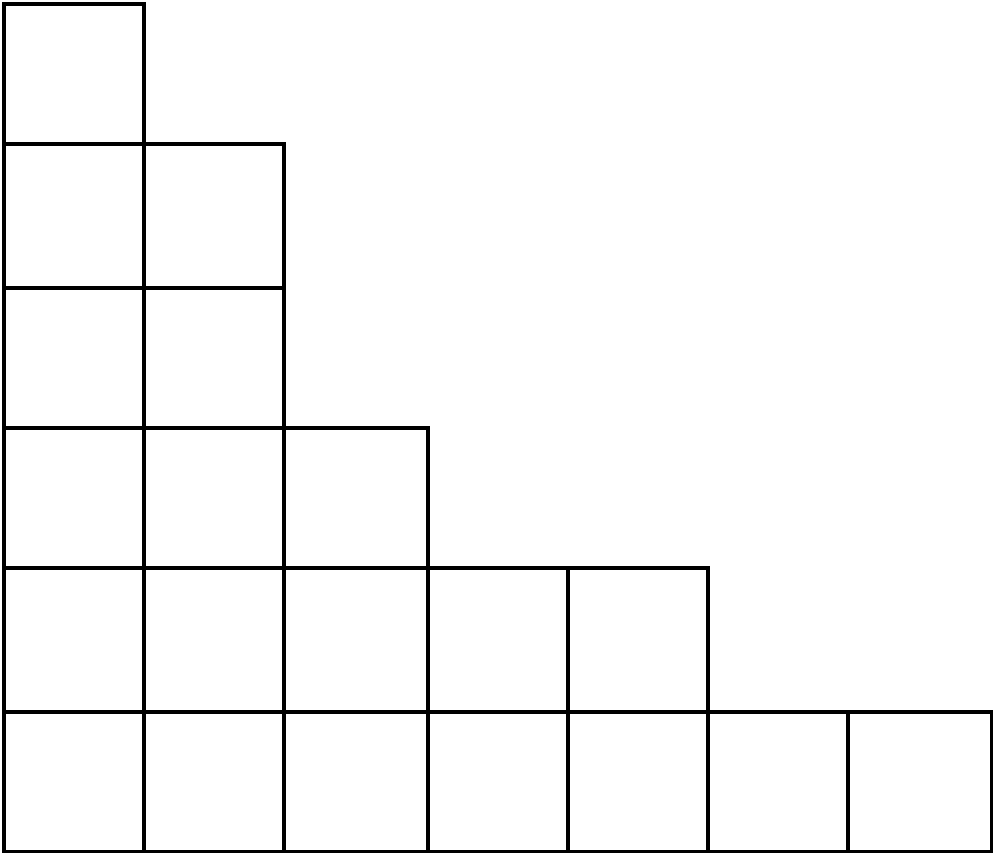
\includegraphics[width=0.5\linewidth]{Images/Figure17.png}
    \caption{The Ferrer's diagram for $7+5+3+2+2+1$}
\end{figure}
It is clear that height of the Ferrer's diagram corresponds to the number of parts in the partition and that the width corresponds to the size of the largest part in the partition. To this end, consider the following result. 
\begin{theorem}
The  number of partitions of $n$ into atmost $i$ parts, each of which is atmost $j$ is the same as the number of partitions of $n$ into atmost $j$ parts, each of which is atmost $i$. 
\end{theorem}
\begin{proof}
Let $\pi$ a partition of $n$ into atmost $i$ parts each of which is atmost $j$. The Ferrer's diagram corresponding to $\pi$ now has height atmost $i$ and width atmost $j$. Flipping the said diagram about it's main diagonal results in a diagram which has height atmost $j$ and width atmost $i$. Finally, the partition corresponding to this flipped diagram (called the conjugate partition) is a partition of $n$ into atmost $j$ parts, each of which is atmost $i$. 
\end{proof}
\begin{figure}[H]
    \centering
    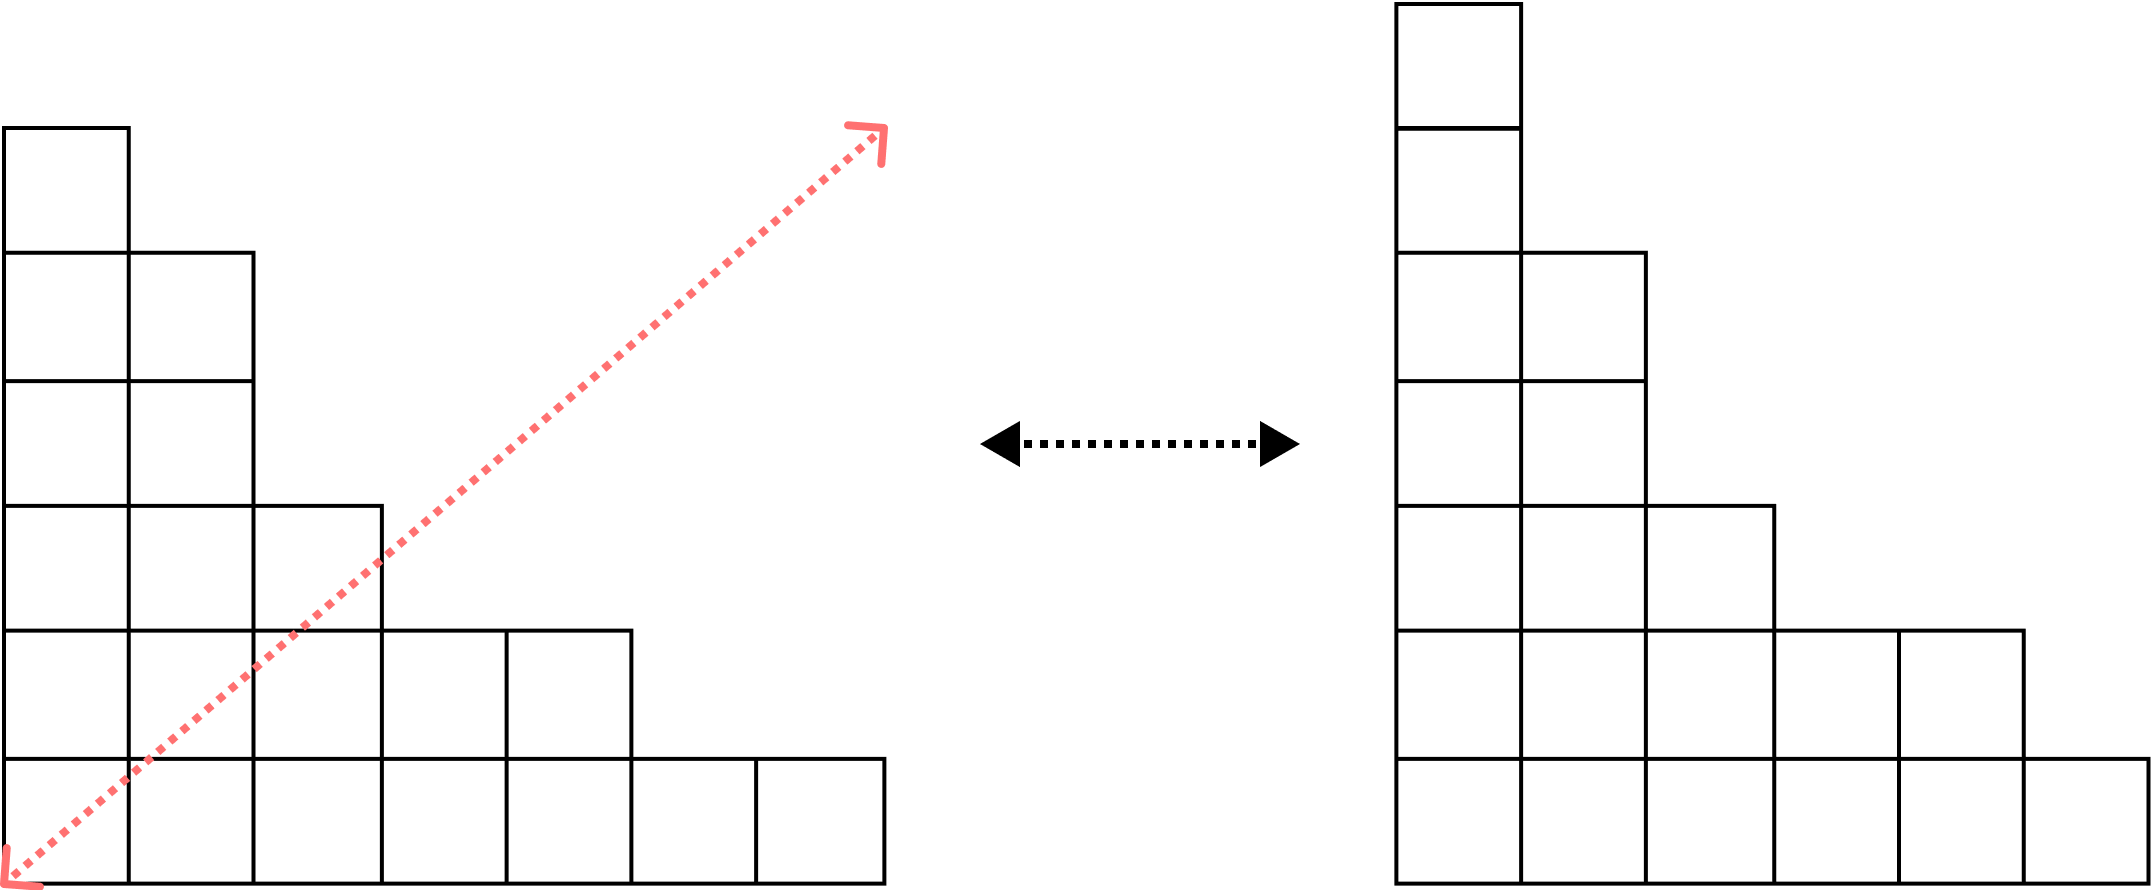
\includegraphics[width=0.8\linewidth]{Images/Figure18.png}
    \caption{An example of the conjugate of $7+5+3+2+2+1$}
\end{figure}
Another useful pictorial construct is that of a Durfee square. We define the said square to be the largest one which can fit in the Ferrer’s diagram corresponding to a partition.
\begin{figure}[H]
    \centering
    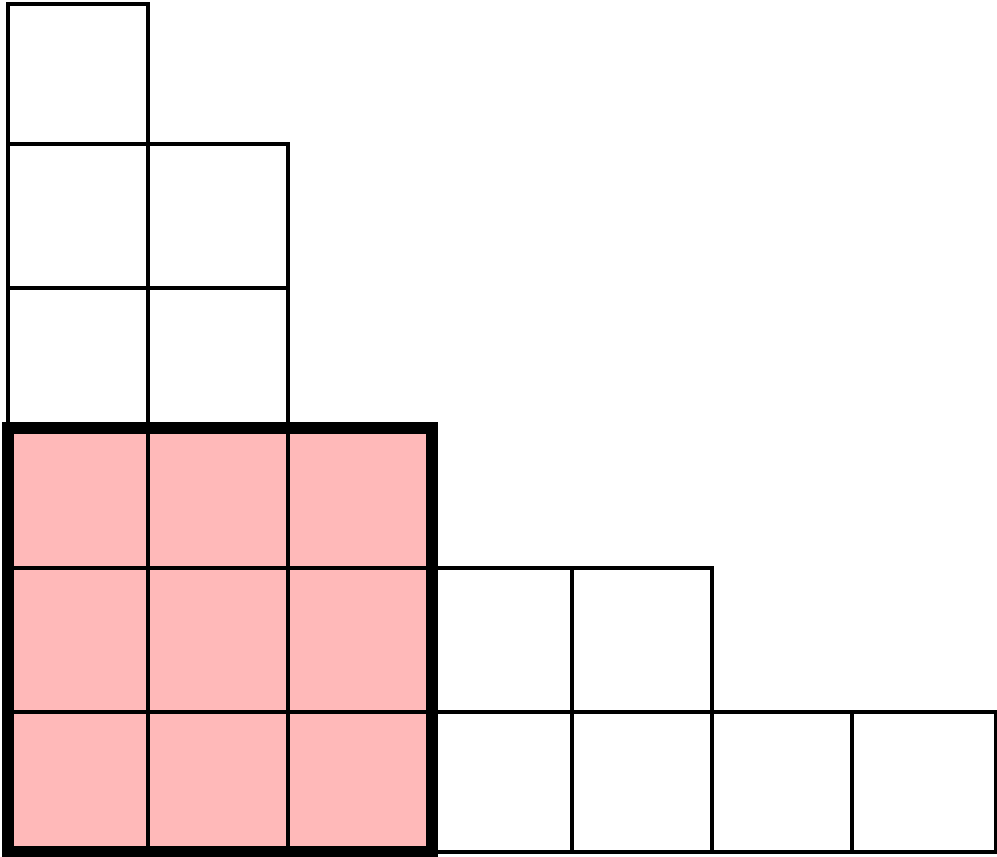
\includegraphics[width=0.5\linewidth]{Images/Figure19.png}
    \caption{The Durfee square of order $3$ in the partition $7+5+3+2+2+1$}
    \label{DurfeeExample}
\end{figure}
(Keeping in mind \cref{DurfeeExample}) notice how
\begin{enumerate}
    \item Every non-empty partition has a Durfee square of order $k$ (if nothing, you always have the Durfee square of order $k=1$).
    \item Partitions corresponding to the triangle above the Durfee square are the ones where each part is atmost $k$.
    \item Partitions corresponding to the triangle below the Durfee square are the ones where number of parts are atmost $k$. 
\end{enumerate}
With these three observations at hand, an identity presents itself almost immediately. Namely,
\begin{claim}
    \[
    \prod_{i=1}^{\infty}\dfrac{1}{1-q^i} = \sum_{i=0}^{\infty}\dfrac{q^{i^2}}{(1-q)^2(1-q^2)^2\cdots(1-q^i)^2}
    \]
\end{claim}
\begin{theorem}[Euler's Pentagonal Number Theorem]
\begin{align*}
\prod_{i=1}^{n}(1-q^i) &= \sum_{k=-\infty}^{\infty}(-1)^k q^{\dfrac{k(3k-1)}{2}} \\
&= 1+\sum_{k=1}^{\infty}(-1)^kq^{\dfrac{k(3k-1)}{2}}+\sum_{k=-\infty}^{-1}(-1)^kq^{\dfrac{k(3k-1)}{2}} \\
&= 1+\sum_{k=1}^{\infty}(-1)^kq^{\dfrac{k(3k-1)}{2}}+\sum_{k=1}^{\infty}(-1)^kq^{\dfrac{k(3k+1)}{2}} \\
&= 1+\sum_{k=1}^{\infty}(-1)^k \left(q^{\dfrac{k(3k-1)}{2}}+q^{\dfrac{k(3k+1)}{2}}\right) \\
\end{align*}
\end{theorem}
%Give a proof using the bi-variate generating 

\endinput
